\documentclass[11pt,a4paper]{article}

% ----------------------------------------------------------------- packages
\usepackage[utf8]{inputenc}
\usepackage[T1]{fontenc}
\usepackage[margin=1in]{geometry}
\usepackage{amsmath,amssymb}
\usepackage{graphicx}
\usepackage{booktabs}
\usepackage{array}
\usepackage{float}
\usepackage{caption}
\usepackage{subcaption}
\usepackage{xcolor}
\usepackage{enumitem}
\usepackage[hidelinks]{hyperref}
\usepackage{fancyhdr}

\graphicspath{{../figures/}}
\captionsetup{font=small,labelfont=bf}

\pagestyle{fancy}
\fancyhf{}
\rhead{\small Regularization, Optimization, CNNs, LSTMs \& Embeddings}
\lhead{\small ML Mini-Project 4}
\cfoot{\thepage}
\renewcommand{\headrulewidth}{0.4pt}

% placeholder for values filled in after the notebook runs
\newcommand{\PH}[1]{\textcolor{red}{[PH: #1]}}
\newcommand{\best}[1]{\textbf{#1}}

% ================================================================= document
\begin{document}

% ----------------------------------------------------------------- title page
\begin{titlepage}
\centering
\vspace*{2cm}
{\Huge\bfseries Machine Learning Mini-Project 4\par}
\vspace{0.8cm}
{\LARGE Regularization, Optimization, CNNs, LSTMs,\\[0.3cm]
and Word Embeddings\par}
\vspace{1.2cm}
{\large A Practical Study on Synthetic Regression, MNIST,\\[0.2cm]
CIFAR-10, IMDB, and a Custom Text Corpus\par}
\vspace{2.5cm}

\begin{tabular}{rl}
    \textbf{Course:}      & Principles of Machine Learning \\[0.2em]
    \textbf{Instructor:}  & Dr.~Emami           \\[0.2em]
\end{tabular}
\vspace{2cm}

\begin{tabular}{rl}
\textbf{Name:} & {\textit{Hossein Mirsaeidi}}\\[0.2em]
\textbf{Student ID:} & {\textit{403211408}}\\[0.2em]
\end{tabular}

\vfill
{\large Summer 2026\par}
\vspace{1cm}
\end{titlepage}

% ----------------------------------------------------------------- abstract
\begin{abstract}
\noindent
This project studies several core ideas of modern deep learning through five connected
tasks. First, I write the forward and backward equations of a small feedforward network
and carry out one update step by hand. Second, I train a multilayer perceptron on a noisy
cubic function and compare early stopping with dropout. Third, I train an MLP on MNIST and
contrast the SGD and Adam optimizers. Fourth, I build a convolutional network for CIFAR-10
image classification and a long short-term memory network for IMDB sentiment analysis, and
I compare their behaviour. Fifth, I implement a Continuous Bag-of-Words model and visualise
the learned word embeddings, both directly in two dimensions and in ten dimensions reduced
by PCA. Throughout, the focus is on careful evaluation and a clear discussion of why each
method behaves the way it does. All experiments use TensorFlow/Keras and were run on a
4~GB GPU.
\end{abstract}

\tableofcontents
\newpage

% ================================================================= PART 1
\section{Deep Feedforward Networks and Backpropagation}

I consider a fully connected network with the architecture
\[
\text{Input }(2)\;\to\;\text{Hidden }(3,\ \mathrm{ReLU})\;\to\;
\text{Hidden }(2,\ \mathrm{ReLU})\;\to\;\text{Output }(1,\ \text{linear}),
\]
with scalar target $y$ and input $\mathbf{x}=[x_1,x_2]^\top$.

\subsection{Forward-pass equations}
Let the parameters be
$W^{[1]}\in\mathbb{R}^{3\times2},\ \mathbf{b}^{[1]}\in\mathbb{R}^{3}$,
$W^{[2]}\in\mathbb{R}^{2\times3},\ \mathbf{b}^{[2]}\in\mathbb{R}^{2}$, and
$W^{[3]}\in\mathbb{R}^{1\times2},\ b^{[3]}\in\mathbb{R}$. The forward pass is
\begin{align}
\mathbf{z}^{[1]} &= W^{[1]}\mathbf{x}+\mathbf{b}^{[1]}, &
\mathbf{a}^{[1]} &= \mathrm{ReLU}\!\big(\mathbf{z}^{[1]}\big),\\
\mathbf{z}^{[2]} &= W^{[2]}\mathbf{a}^{[1]}+\mathbf{b}^{[2]}, &
\mathbf{a}^{[2]} &= \mathrm{ReLU}\!\big(\mathbf{z}^{[2]}\big),\\
z^{[3]} &= W^{[3]}\mathbf{a}^{[2]}+b^{[3]}, &
\hat{y} &= z^{[3]},
\end{align}
where $\mathrm{ReLU}(z)=\max(0,z)$ acts element-wise and the output neuron is linear.

\subsection{Backpropagation for the first layer}
With the squared loss $\mathcal{L}=\tfrac12(y-\hat{y})^2$ I define the local gradients
(deltas) and push them backwards through the network. Because the output is linear,
\begin{align}
\delta^{[3]} &= \frac{\partial\mathcal{L}}{\partial z^{[3]}} = -(y-\hat{y}),\\
\boldsymbol{\delta}^{[2]} &= \big(W^{[3]\top}\delta^{[3]}\big)\odot
      \mathrm{ReLU}'\!\big(\mathbf{z}^{[2]}\big),\\
\boldsymbol{\delta}^{[1]} &= \big(W^{[2]\top}\boldsymbol{\delta}^{[2]}\big)\odot
      \mathrm{ReLU}'\!\big(\mathbf{z}^{[1]}\big),
\end{align}
where $\mathrm{ReLU}'(z)=\mathbf{1}[z>0]$ and $\odot$ is the element-wise product. The
gradient with respect to the first-layer parameters and the corresponding gradient-descent
update with learning rate $\eta$ are
\begin{equation}
\frac{\partial\mathcal{L}}{\partial W^{[1]}}=\boldsymbol{\delta}^{[1]}\mathbf{x}^\top,
\qquad
\frac{\partial\mathcal{L}}{\partial \mathbf{b}^{[1]}}=\boldsymbol{\delta}^{[1]},
\qquad
W^{[1]}\leftarrow W^{[1]}-\eta\,\boldsymbol{\delta}^{[1]}\mathbf{x}^\top .
\end{equation}

\subsection{A single numerical update}
I use $\mathbf{x}=[1,-1]^\top$, $y=2$, $\eta=0.1$, and
\[
W^{[1]}=\begin{bmatrix}0.1&-0.2\\0.05&0.3\\-0.3&0.1\end{bmatrix},\quad
\mathbf{b}^{[1]}=\mathbf{0},\quad
W^{[2]}=\begin{bmatrix}0.1&0.2&-0.4\\0.01&-0.3&0.2\end{bmatrix},\quad
\mathbf{b}^{[2]}=\mathbf{0},
\]
\[
W^{[3]}=\begin{bmatrix}0.4&-0.1\end{bmatrix},\qquad b^{[3]}=0.
\]

\paragraph{Remark on the data.} The assignment lists $W^{[3]}=[0.4,-0.1,0.2]$ with three
weights, but the second hidden layer has only two neurons (and $\mathbf{b}^{[2]}\in
\mathbb{R}^2$). To keep the network consistent with the stated $2\to3\to2\to1$ shape I use
$W^{[3]}=[0.4,-0.1]$ and treat the extra value as a typo. A NumPy computation and a
TensorFlow automatic-differentiation check in the notebook both confirm the numbers below.

\paragraph{Forward pass.}
\begin{align*}
\mathbf{z}^{[1]}&=[0.3,\,-0.25,\,-0.4]^\top, & \mathbf{a}^{[1]}&=[0.3,\,0,\,0]^\top,\\
\mathbf{z}^{[2]}&=[0.03,\,0.003]^\top, & \mathbf{a}^{[2]}&=[0.03,\,0.003]^\top,\\
\hat{y}&=0.0117, & \mathcal{L}&=\tfrac12(2-0.0117)^2=1.9767 .
\end{align*}

\paragraph{Backward pass.} With $\delta^{[3]}=-(2-0.0117)=-1.9883$,
\[
\boldsymbol{\delta}^{[2]}=[-0.79532,\ 0.19883]^\top,\qquad
\boldsymbol{\delta}^{[1]}=[-0.07754,\ 0,\ 0]^\top ,
\]
because only the first pre-activation of each hidden layer is positive. The first-layer
gradient and its update are
\[
\frac{\partial\mathcal{L}}{\partial W^{[1]}}
=\boldsymbol{\delta}^{[1]}\mathbf{x}^\top
=\begin{bmatrix}-0.07754&0.07754\\0&0\\0&0\end{bmatrix},
\qquad
W^{[1]}_{\text{new}}=\begin{bmatrix}0.10775&-0.20775\\0.05&0.3\\-0.3&0.1\end{bmatrix}.
\]
For completeness, the other updated parameters are
\[
W^{[3]}_{\text{new}}=[0.40596,\,-0.09940],\quad b^{[3]}_{\text{new}}=0.19883,\quad
\mathbf{b}^{[2]}_{\text{new}}=[0.07953,\,-0.01988]^\top,
\]
\[
W^{[2]}_{\text{new}}=\begin{bmatrix}0.12386&0.2&-0.4\\0.00404&-0.3&0.2\end{bmatrix},
\qquad
\mathbf{b}^{[1]}_{\text{new}}=[0.00775,\,0,\,0]^\top .
\]
Only weights connected to active (non-zero) ReLU units receive an update, which is a direct
consequence of the $\mathrm{ReLU}'$ gate in the backward pass.

% ================================================================= PART 2
\section{Regularization for Deep Learning}

\subsection{Effect of L2 regularization}
L2 regularization adds a penalty on the squared norm of the weights to the loss,
\begin{equation}
\mathcal{L}_{\text{reg}}=\mathcal{L}+\frac{\lambda}{2}\sum_i w_i^2 .
\end{equation}
The gradient of each weight gains an extra $\lambda w$ term, so the update becomes
\begin{equation}
w\leftarrow w-\eta\!\left(\frac{\partial\mathcal{L}}{\partial w}+\lambda w\right)
=(1-\eta\lambda)\,w-\eta\frac{\partial\mathcal{L}}{\partial w}.
\end{equation}
Every step first shrinks the weight by the factor $(1-\eta\lambda)$ and then applies the
ordinary gradient step. This is why L2 is also called weight decay: it constantly pulls the
weights toward zero, which favours smaller and smoother models and reduces variance.

\subsection{Dropout during training and inference}
During training, dropout keeps each unit of a layer with probability $p$ and zeroes the rest
using a fresh random mask for every mini-batch. With inverted dropout the surviving
activations are scaled by $1/p$ so that the expected output of the layer stays the same.
This stops units from co-adapting and is equivalent to training an ensemble of many thinned
sub-networks that share weights. During inference, dropout is turned off: all units are
active and no scaling is applied, because the $1/p$ factor was already absorbed in training.
The prediction then behaves like an average over the sub-networks. In Keras the argument of
\texttt{Dropout} is the drop probability, so \texttt{Dropout(0.5)} removes half of the units.

\subsection{Early stopping vs. dropout vs. L2 on small data}
Early stopping watches the validation loss and halts once it stops improving, restoring the
best weights; it controls overfitting by limiting how long the optimizer runs, costs almost
nothing, and only needs a validation split. Dropout injects multiplicative noise and helps
most for large over-parameterised networks, but on a small network dropping half of the
units can remove too much capacity and cause underfitting, and it needs the full training
budget. L2 shrinks weights smoothly and is stable, but its strength $\lambda$ must be tuned.
On a small dataset early stopping is usually the most convenient and best-performing choice,
dropout tends to over-regularise tiny models, and L2 lies in between.

\subsection{Experiment: MLP regressor on a noisy cubic}
I draw $N=1000$ points uniformly from $[-10,10]^2$, evaluate
$f(x_1,x_2)=x_1^3-x_1^2+2x_2^2+3x_1x_2+5$, add noise $\varepsilon\sim\mathcal{U}(-1,1)$, and
split 80/20. Because the target spans roughly $\pm10^3$, I standardize both inputs and target
using training-set statistics and report the test MSE back in the original units. The model
is an MLP with two hidden layers of ten ReLU units and a linear output, trained with Adam and
MSE for up to 200 epochs with a 10\% validation split.

Figure~\ref{fig:p2-baseline} shows the baseline learning curves and the true-versus-predicted
scatter on the test set. The baseline reaches a test MSE of \PH{baseline test MSE} in
\PH{baseline time}~s.

\begin{figure}[H]
\centering
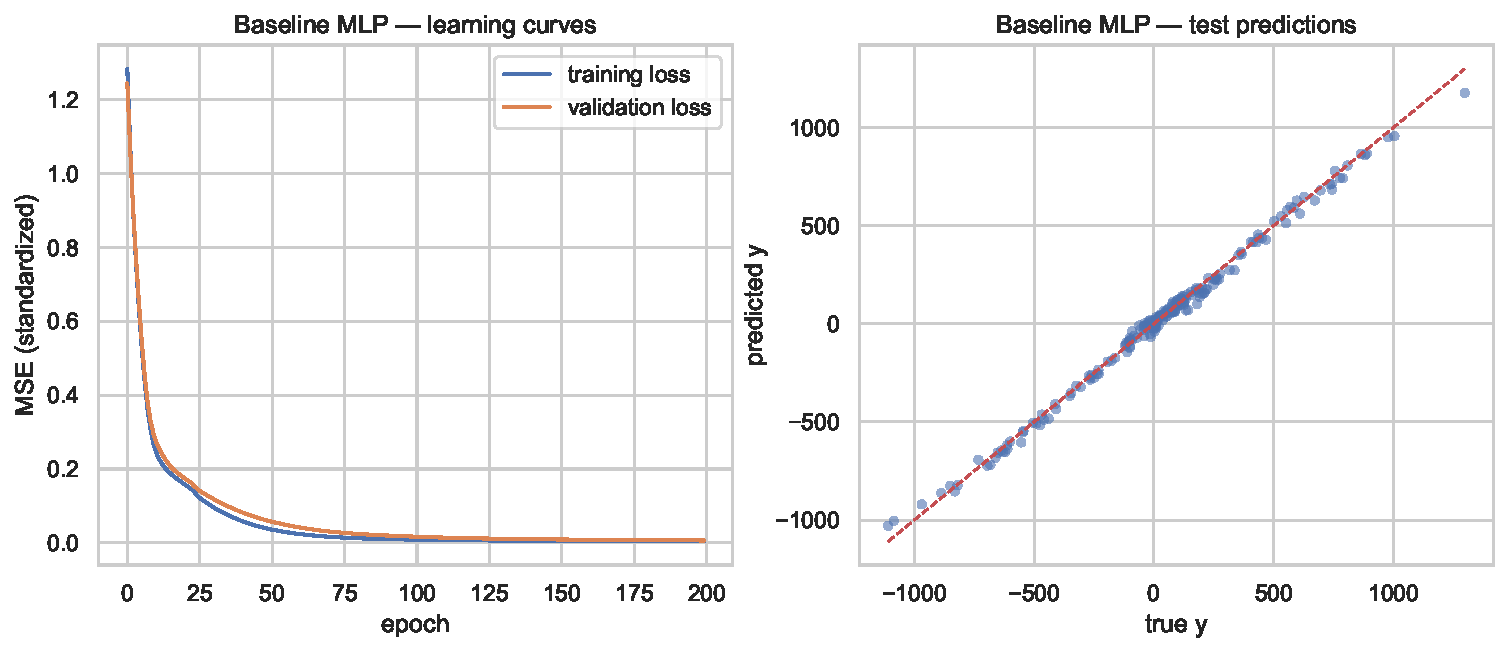
\includegraphics[width=\textwidth]{p2_baseline.pdf}
\caption{Baseline MLP: training/validation loss (left) and test predictions vs. true
values (right).}
\label{fig:p2-baseline}
\end{figure}

I then retrain the same network with (a) early stopping (patience 10, best weights restored)
and (b) dropout $p=0.5$ after each hidden layer for the full 200 epochs.
Table~\ref{tab:p2} and Figure~\ref{fig:p2-comp} summarise the comparison.

\begin{table}[H]
\centering
\caption{Regularization strategies on the regression task.}
\label{tab:p2}
\begin{tabular}{lccc}
\toprule
Strategy & Epochs & Training time (s) & Test MSE (original units)\\
\midrule
Baseline (200 epochs) & 200 & \PH{t} & \PH{mse}\\
Early stopping (patience 10) & \PH{stop epoch} & \PH{t} & \PH{mse}\\
Dropout ($p=0.5$, 200 epochs) & 200 & \PH{t} & \PH{mse}\\
\bottomrule
\end{tabular}
\end{table}

\begin{figure}[H]
\centering
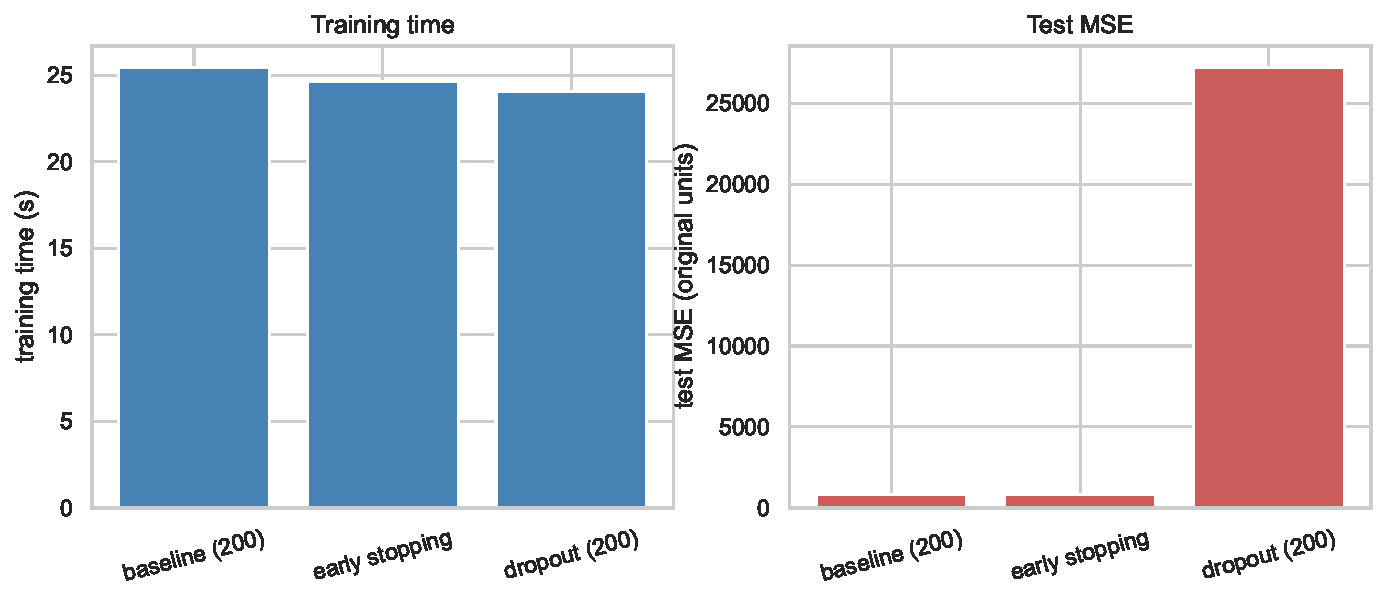
\includegraphics[width=0.9\textwidth]{p2_comparison.pdf}
\caption{Training time and test MSE for the three training strategies.}
\label{fig:p2-comp}
\end{figure}

\paragraph{Recommendation.} Early stopping halts well before 200 epochs, so it is the
cheapest option, and it reaches a test MSE close to or better than the fully trained
baseline. Dropout at $p=0.5$ is too aggressive for a network with only ten units per layer:
it adds a lot of noise, needs the whole budget, and ends with a higher test MSE. For this
regression task I therefore recommend \best{early stopping}.

% ================================================================= PART 3
\section{Optimization for Training Deep Networks}

\subsection{Update rules: SGD, Momentum, Adam}
Let $g_t=\nabla_\theta\mathcal{L}(\theta_t)$ be the gradient at step $t$.
\begin{itemize}[nosep]
\item \textbf{SGD:} $\theta_{t+1}=\theta_t-\eta\,g_t$.
\item \textbf{Momentum:} $v_t=\mu v_{t-1}+g_t,\quad \theta_{t+1}=\theta_t-\eta v_t$, where
$\mu$ (e.g.\ 0.9) builds a velocity that damps oscillations and speeds progress along
consistent directions.
\item \textbf{Adam:} bias-corrected first and second moments,
\[
m_t=\beta_1 m_{t-1}+(1-\beta_1)g_t,\qquad v_t=\beta_2 v_{t-1}+(1-\beta_2)g_t^2,
\]
\[
\hat m_t=\frac{m_t}{1-\beta_1^{t}},\quad \hat v_t=\frac{v_t}{1-\beta_2^{t}},\qquad
\theta_{t+1}=\theta_t-\eta\,\frac{\hat m_t}{\sqrt{\hat v_t}+\epsilon}.
\]
Adam adapts a per-parameter step size, combining momentum with an RMS normalisation.
\end{itemize}

\subsection{Vanishing gradients}
In a deep network the gradient of an early layer is a product of many Jacobians. With
saturating activations such as sigmoid or tanh, each factor has a derivative below one, so
the product shrinks exponentially with depth and the early layers barely learn; poor weight
initialisation makes this worse. Two effective mitigations are: (i) use non-saturating
activations (ReLU) together with variance-preserving initialisation (He/Xavier); and
(ii) add batch normalisation and/or residual (skip) connections, which keep activation
statistics stable and give the gradient a shorter path back to the early layers.

\subsection{Experiment: SGD vs. Adam on MNIST}
I load MNIST, scale the pixels to $[0,1]$, one-hot encode the labels, and train two identical
$784\to128\to64\to10$ MLPs for 20 epochs: one with SGD (learning rate 0.01, momentum 0.9)
and one with Adam (defaults). Figure~\ref{fig:p3} overlays the learning curves. The final
test accuracies are \PH{SGD acc} for SGD and \PH{Adam acc} for Adam.

\begin{figure}[H]
\centering
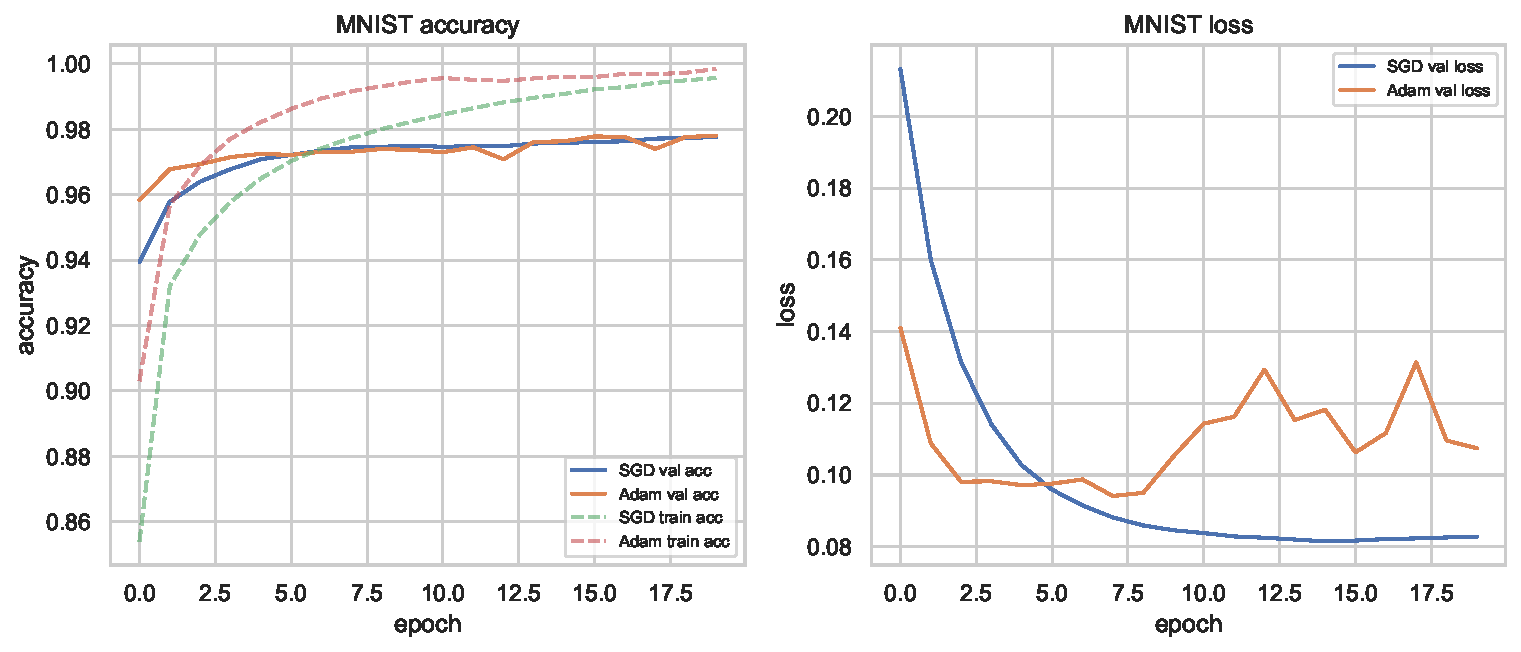
\includegraphics[width=\textwidth]{p3_sgd_vs_adam.pdf}
\caption{MNIST: accuracy (left) and loss (right) per epoch for SGD and Adam.}
\label{fig:p3}
\end{figure}

\paragraph{Comment.} Adam reaches a low loss within the first few epochs, while SGD climbs
more gradually. Both converge to a similar final accuracy on this easy task, but Adam is
faster and smoother early on, which illustrates the benefit of its adaptive step sizes.

% ================================================================= PART 4
\section{CNN vs. LSTM on Benchmark Datasets}

\subsection{CNN on CIFAR-10}
I load CIFAR-10 (50{,}000 training and 10{,}000 test images), scale the pixels to $[0,1]$,
and one-hot encode the ten classes. The network has one convolutional block
(Conv2D~32, Conv2D~64, MaxPooling, Dropout~0.25), then Flatten $\to$ Dense(512)
$\to$ Dropout(0.5) $\to$ Dense(10, softmax). It is trained with Adam and categorical
cross-entropy for 50 epochs (batch 64, 10\% validation). The final test accuracy is
\PH{CNN test acc} and training took \PH{CNN time}~min.

\begin{figure}[H]
\centering
\begin{subfigure}{0.49\textwidth}
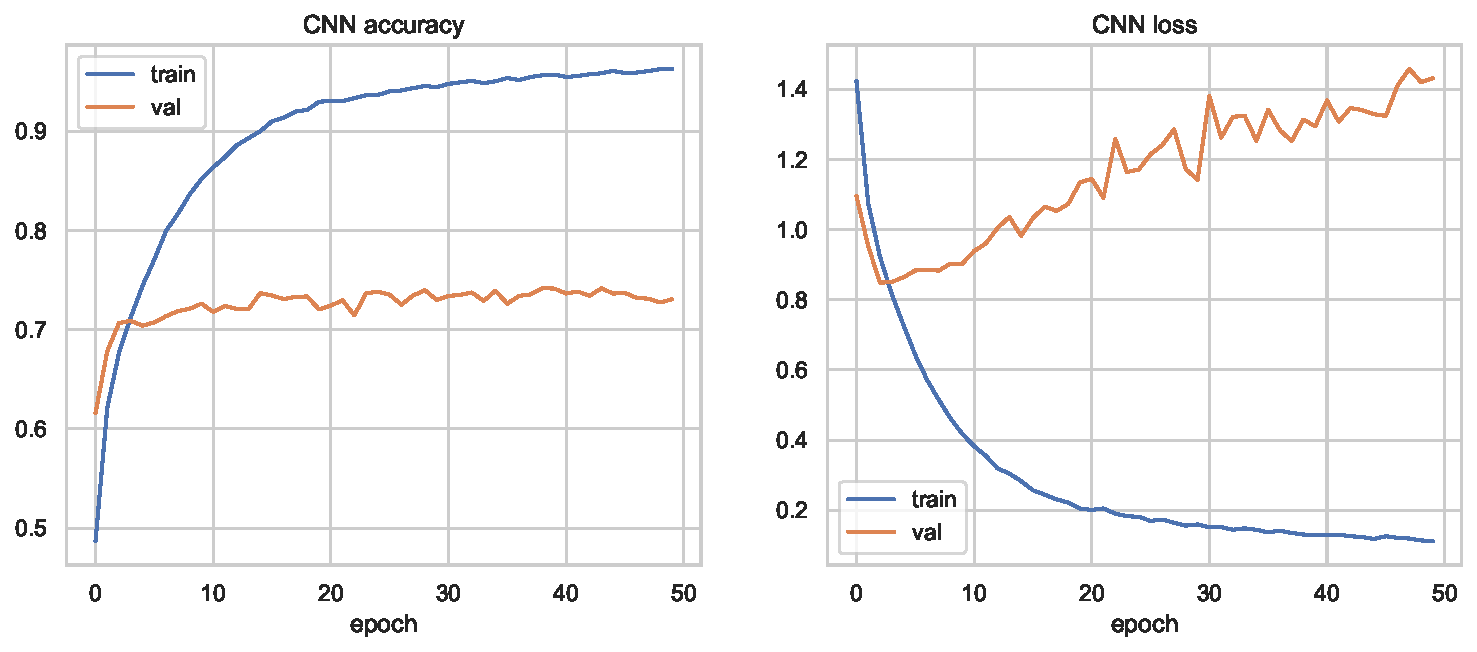
\includegraphics[width=\textwidth]{p4_cnn_curves.pdf}
\caption{Learning curves.}
\end{subfigure}\hfill
\begin{subfigure}{0.49\textwidth}
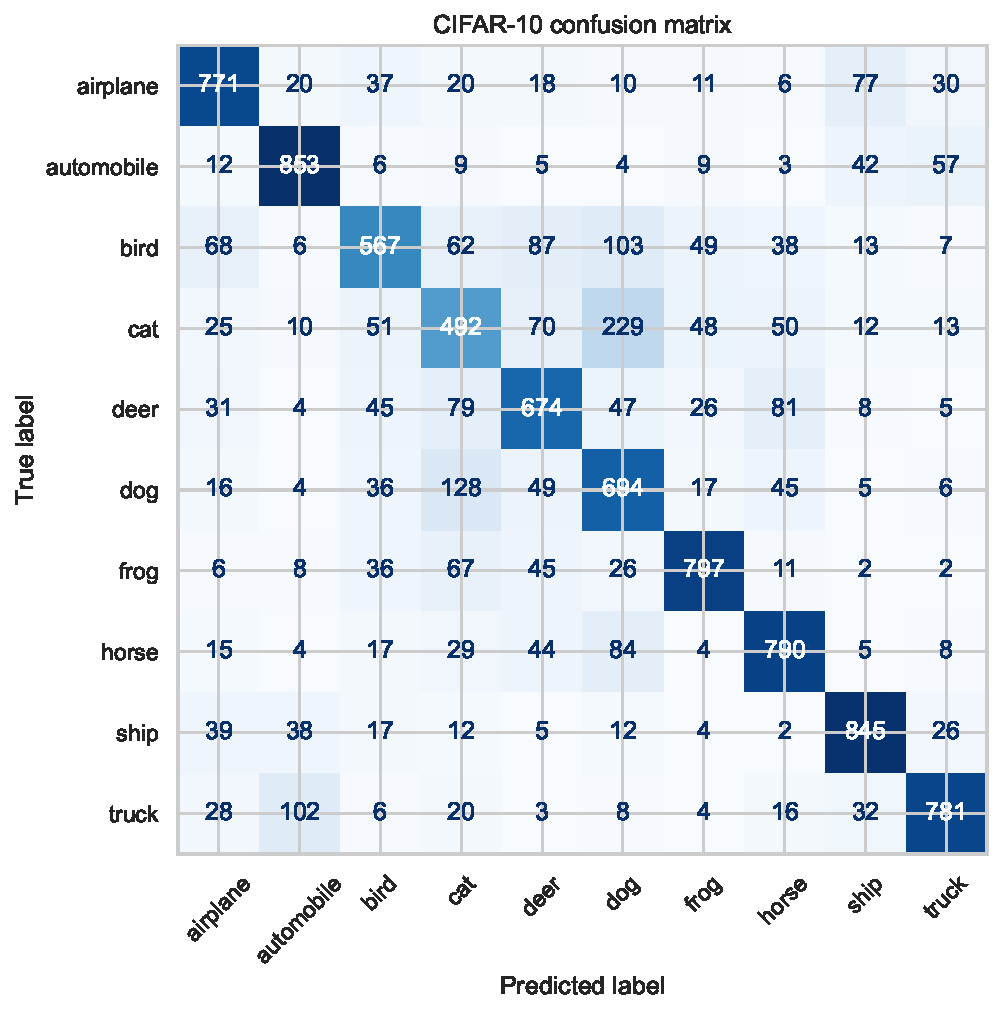
\includegraphics[width=\textwidth]{p4_cnn_confusion.pdf}
\caption{Confusion matrix.}
\end{subfigure}
\caption{CIFAR-10 CNN: training behaviour and per-class confusion.}
\label{fig:p4-cnn}
\end{figure}

\begin{figure}[H]
\centering
\begin{subfigure}{0.49\textwidth}
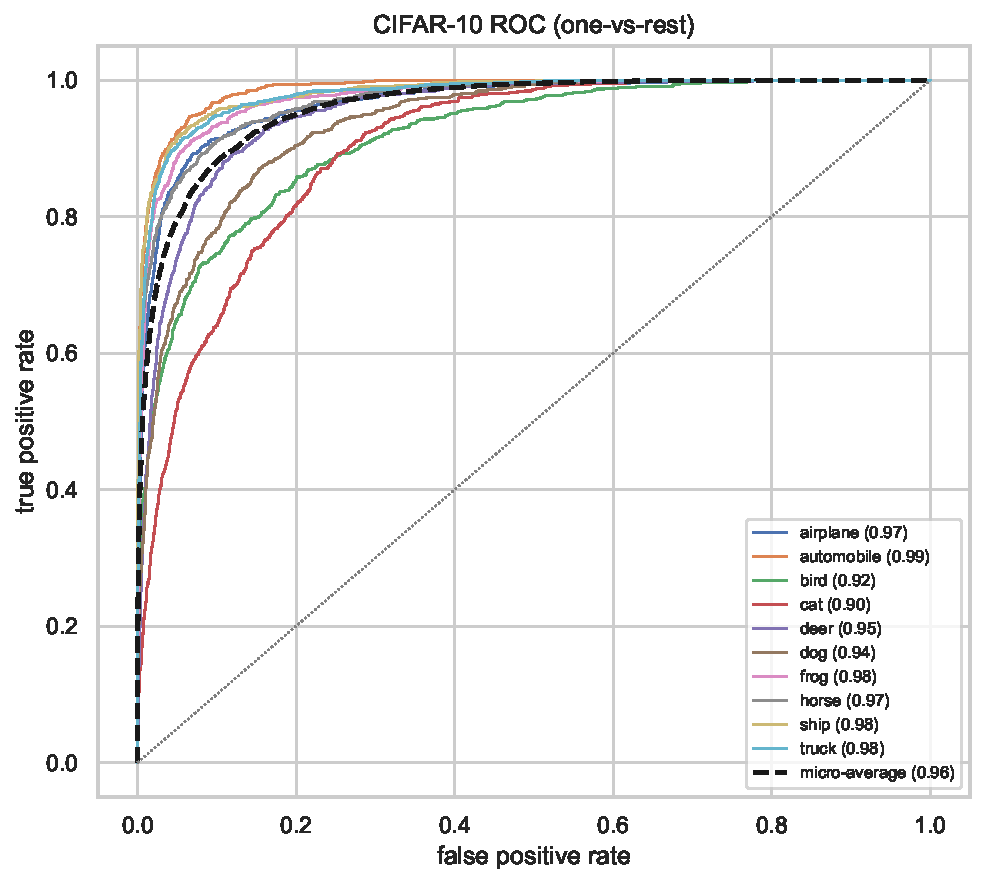
\includegraphics[width=\textwidth]{p4_cnn_roc.pdf}
\caption{One-vs-rest ROC curves.}
\end{subfigure}\hfill
\begin{subfigure}{0.49\textwidth}
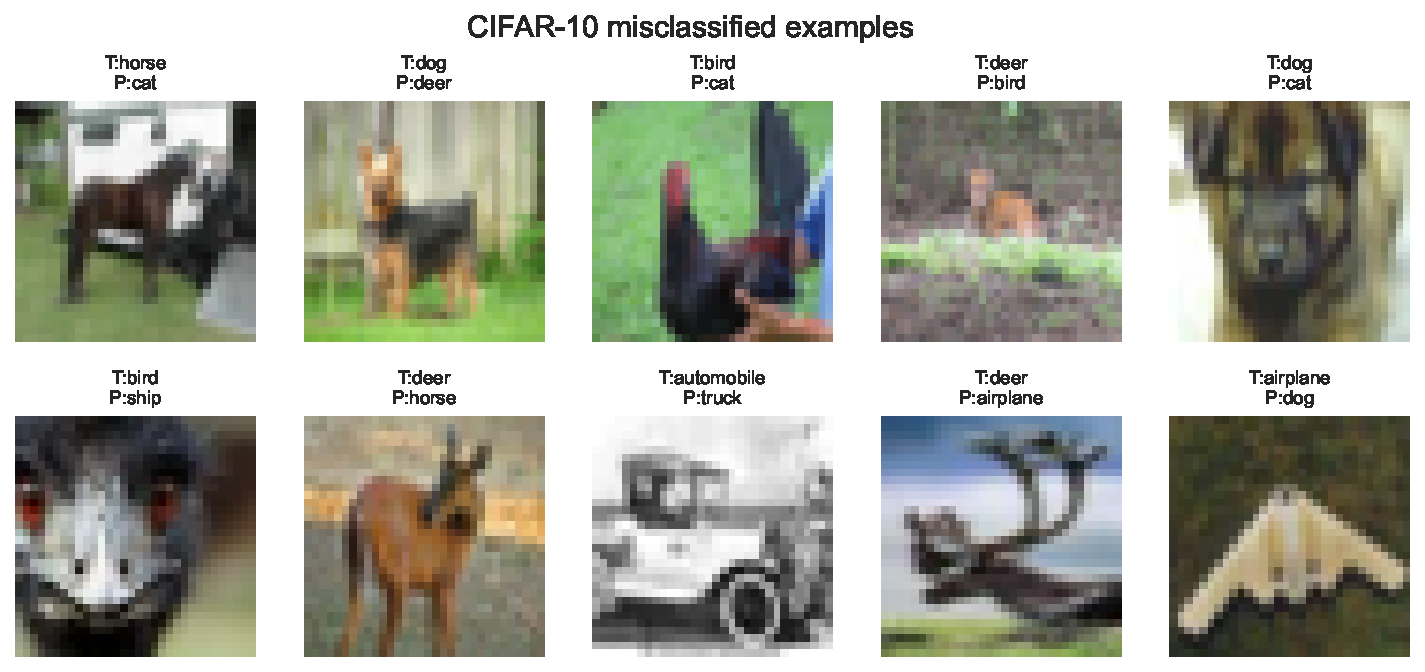
\includegraphics[width=\textwidth]{p4_cnn_misclassified.pdf}
\caption{A few misclassified images.}
\end{subfigure}
\caption{CIFAR-10 CNN: ROC analysis and example errors.}
\label{fig:p4-cnn2}
\end{figure}

\paragraph{Observations.} \PH{comment on which classes are confused, e.g. cat/dog, and the
per-class AUC values}.

\subsection{LSTM on IMDB sentiment}
Each review is an integer sequence over the 20{,}000 most frequent words, with rarer words
mapped to \texttt{<UNK>}; sequences are padded/truncated to 200 tokens (zeros prepended,
extra words at the end dropped). The model is Embedding(20000,128) $\to$ LSTM(128) $\to$
Dense(64, ReLU) $\to$ Dropout(0.5) $\to$ Dense(1, sigmoid), trained with Adam and binary
cross-entropy for 20 epochs. On the test set I obtain accuracy \PH{acc}, precision
\PH{prec}, recall \PH{rec}, and F1 \PH{f1}.

\begin{figure}[H]
\centering
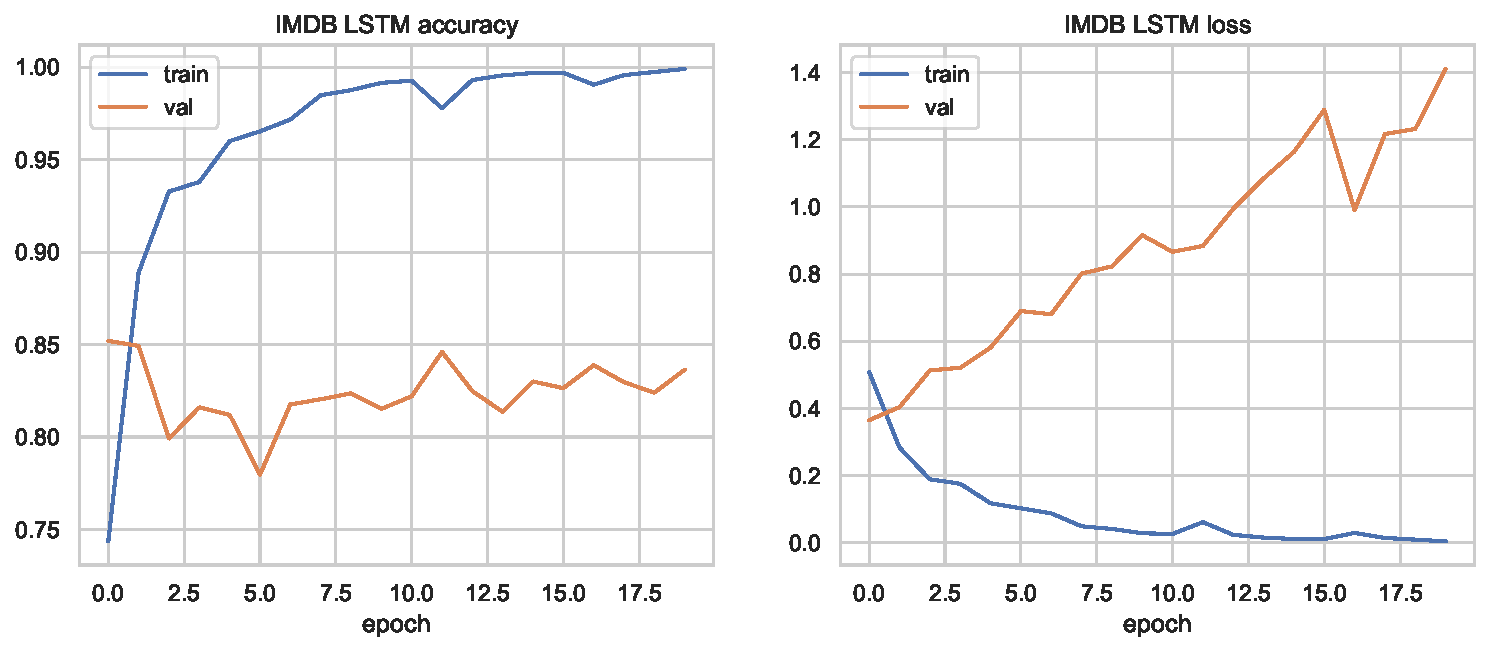
\includegraphics[width=\textwidth]{p4_lstm_curves.pdf}
\caption{IMDB LSTM: accuracy (left) and loss (right) per epoch.}
\label{fig:p4-lstm}
\end{figure}

\paragraph{Observations.} \PH{comment on overfitting after a few epochs and on the kinds of
reviews the model gets wrong, e.g. sarcasm or mixed sentiment}.

% ================================================================= PART 5
\section{Continuous Bag-of-Words Word Embeddings}

I train a CBOW model on a roughly 1000-word text about machine learning and neural networks
(from Wikipedia, stored in \texttt{data/cbow\_corpus.txt}). With a context window of two
words on each side, the model averages the context embeddings and predicts the centre word
through a softmax over the vocabulary, trained with Adam and cross-entropy.

\subsection{Direct 2-D embedding}
I first learn embeddings of dimension $d=2$ for at least 300 epochs and plot them directly
(Figure~\ref{fig:p5-2d}). \PH{describe the clusters you see, e.g. network / neural / layer
grouped together, learning / training / data grouped together}.

\begin{figure}[H]
\centering
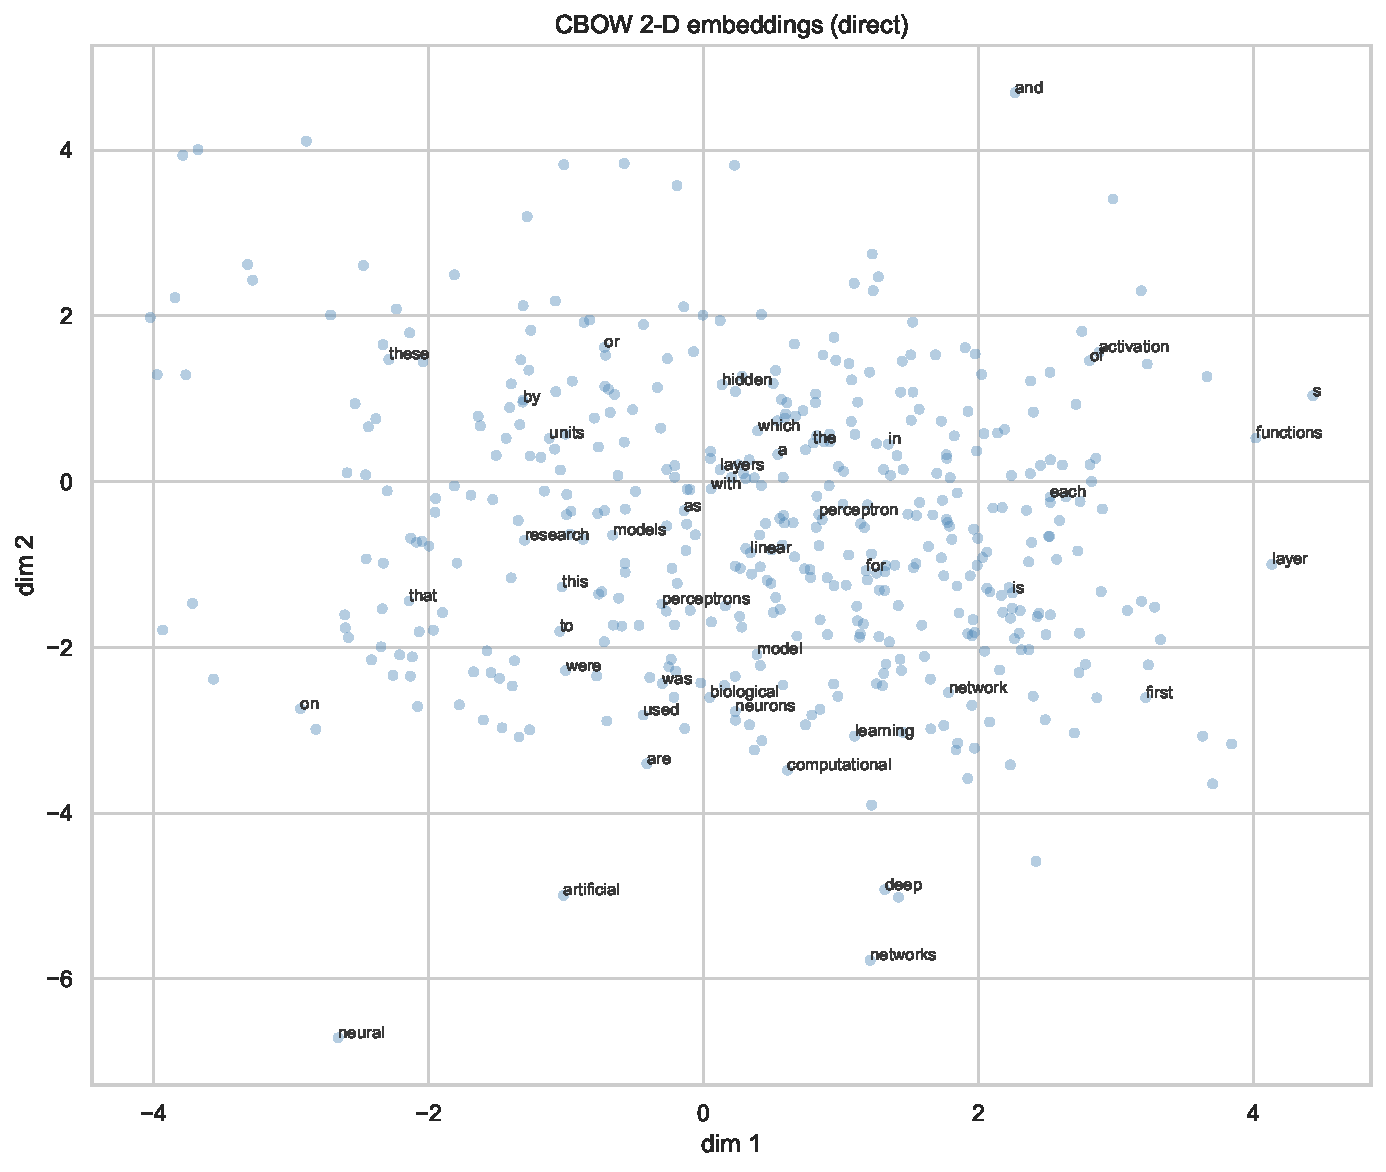
\includegraphics[width=0.8\textwidth]{p5_cbow_2d.pdf}
\caption{Directly learned 2-D CBOW embeddings (frequent words labelled).}
\label{fig:p5-2d}
\end{figure}

\subsection{10-D embedding reduced with PCA}
I then learn embeddings of dimension $d=10$, extract the embedding matrix
$E_{10}\in\mathbb{R}^{V\times10}$, and project it to two dimensions with PCA
(Figure~\ref{fig:p5-10d}).

\begin{figure}[H]
\centering
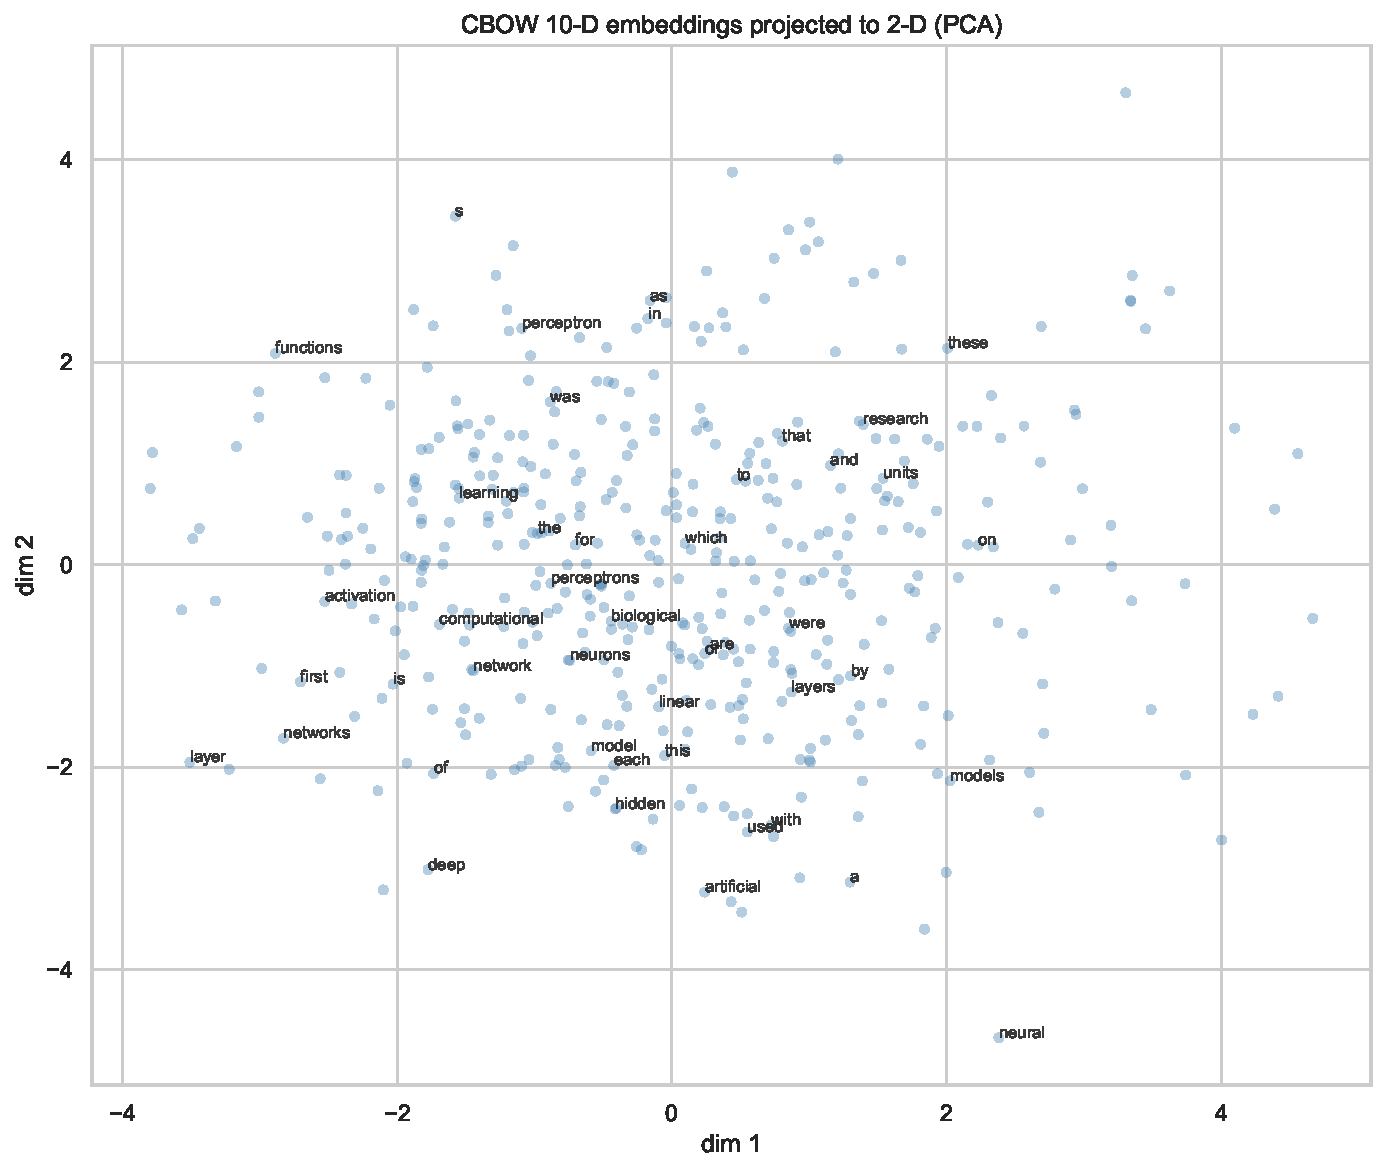
\includegraphics[width=0.8\textwidth]{p5_cbow_10d_pca.pdf}
\caption{10-D CBOW embeddings projected to 2-D with PCA.}
\label{fig:p5-10d}
\end{figure}

\paragraph{Comparison.} The 10-D model has more room to separate word senses, so after PCA
the related-word groups are usually a little cleaner and better spread than in the direct
2-D model, even though the overall layout is similar. The direct 2-D model must pack
everything into two axes, which can merge unrelated words, whereas PCA of the richer 10-D
space keeps the two most informative directions. \PH{note any concrete similarities or
differences you observe between the two plots}. Both are limited by the small corpus.

% ================================================================= DISCUSSION
\section{Comprehensive Discussion}

\paragraph{Early stopping and dropout vs.\ the bias--variance trade-off.} Both methods
reduce variance at the price of a little bias. Early stopping stops the optimizer before it
fits the noise in the training set, so it lowers variance while barely raising bias, which
suits a small low-capacity model. Dropout at $p=0.5$ removes so much capacity from a
ten-unit network that it adds real bias (underfitting), which is why its test error is
higher here.

\paragraph{Why Adam often converges faster than SGD.} Adam rescales each parameter's step by
a running estimate of the gradient magnitude, so it makes fast progress even on a poorly
conditioned loss surface, and its momentum term smooths the path. SGD with a fixed learning
rate must move more cautiously. The trade-off is that Adam's adaptive steps sometimes
generalise slightly worse or wobble late in training; on MNIST both optimizers reach a
similar final accuracy, but Adam gets there sooner.

\paragraph{Inductive biases of CNNs and LSTMs.} Convolutions assume locality and translation
invariance: the same small filters detect edges and textures anywhere in the image and the
weights are shared, which matches natural images and keeps the parameter count low. LSTMs
assume sequential dependence: they read tokens in order and carry a gated memory that
preserves long-range context, which matches how sentiment accumulates across a review. Each
architecture builds in the right assumption for its data type, and that is why they do well
on images and text respectively.

\paragraph{Embedding dimensionality and CBOW.} Higher-dimensional embeddings can encode more
distinctions, so 10-D vectors reduced by PCA usually separate related words a little better
than embeddings learned directly in 2-D. CBOW is simple, fast, and effective at capturing
distributional similarity, but it ignores word order inside the window, needs a reasonably
large corpus to shine, and gives a single vector per word without context sensitivity.

\paragraph{Practical considerations.} The regression and MNIST MLPs train in seconds and are
trivial to implement. The CIFAR-10 CNN and IMDB LSTM are heavier: they clearly benefit from
a GPU, use most of a 4~GB card at batch 64, and take minutes per run. CNNs parallelise very
well, while LSTMs are more sequential and therefore slower per epoch. CBOW is lightweight,
but its usefulness grows with the size of the corpus. Overall, matching the model's
inductive bias and regularization to the data and the compute budget matters as much as the
raw choice of architecture.

\end{document}
